\documentclass[journal]{IEEEtran}

\usepackage[T1]{fontenc}
\usepackage[utf8]{inputenc}
\usepackage{amsmath,amssymb,amsfonts}
\usepackage{amsthm}
\usepackage{graphicx}
\usepackage{array}
\usepackage{url}

\theoremstyle{plain}
\newtheorem{theorem}{Theorem}
\newtheorem{proposition}{Proposition}
\theoremstyle{definition}
\newtheorem{definition}{Definition}
\newtheorem{assumption}{Assumption}
\newtheorem*{remark}{Remark}

\begin{document}

\title{Interaction Dynamics for Floating-Base\\ Whole-Body Manipulation}
\author{Yongyan Cao%
\thanks{Y. Cao. E-mail: yongyancao@gmail.com.}}
\markboth{Manuscript}{Cao: Interaction Dynamics for Floating-Base Whole-Body Manipulation}
\maketitle

\begin{abstract}
Floating-base loco-manipulation is usually split across separate models --- a centroidal predictor, a task-space impedance controller, and a whole-body inverse-dynamics layer beneath them. This paper separates \emph{canonical prediction} from \emph{physical authority}, and anchors that separation on the rate at which each object must actually run. The whole-body feedforward and inverse-dynamics realization form a loop designed for 1 kHz that solves exactly \textbf{one} quadratic program per cycle and never waits on a predictor; body and task requests evolve asynchronously in residual-acceleration coordinates $x_{k+1}=Ax_k+B(u_k+d_k)$ whose exact-ZOH pair $(A,B)$ is invariant to configuration and contact mode. Robot mechanics re-enter not as a second predictive model but as the \emph{admissible geometry} of the command. Because the residual command enters the whole-body QP only through linear cost terms, one KKT solve on the factorization the realizer already computes returns the nominal feedforward and the input maps $K_\tau,K_\lambda$, and the actuator, friction and unilateral limits become linear constraints $H_ku\le h_k$ --- no second optimization. Restricted to the current active set, however, that set is the \emph{critical region}, not the feasible set: it refuses about $68\%$ of feasible commands, falls in $4/4$ single-support transitions, and destroys the task port. Crossing an active-set boundary is not a failure --- the contact forces merely redistribute --- so we \textbf{walk the piecewise-affine solution map}, locating entering and leaving constraints in closed form from the primal and dual blocks of the same KKT system. The walk recovers the exact feasible set (zero false positives \emph{and} zero false negatives) with \textbf{no whole-body QP solves at all}, sustains the support transition $4/4$, and preserves offset-free hand rejection of a sustained interaction force ($364.5\to26.0$ mm, $14\times$). Contact transitions change the admissible command geometry, never the canonical dynamics.
\end{abstract}

\begin{IEEEkeywords}
Interaction dynamics, centroidal MPC, whole-body control, floating-base robots, loco-manipulation, physical human-robot interaction, model predictive control.
\end{IEEEkeywords}

\section{Introduction}\label{sec:introduction}

\IEEEPARstart{H}{umanoid} robots regulate two physical interfaces at once: the feet exchange forces with the environment for balance, the hands with people, tools, and objects for a task. Existing stacks assign these to different objects --- a centroidal MPC plans contact forces, a whole-body QP maps them to joint commands, an impedance controller regulates the hand --- which is practical but hides that both are the same interaction-dynamics problem.

The question here is not whether another whole-body architecture can be assembled, but whether floating-base manipulation admits the same normalized interaction-dynamics representation derived for fixed-base systems in \cite{b1} without making prediction blind to current physical capability. Balance and manipulation should share a canonical predictive representation, while robot-specific mechanics enter through the admissible command geometry and the recovery of normalized requests as physical wrenches. This also serves the emerging \emph{physical-AI} stack: learned policies and world models generate whole-body \emph{intent}, but intent is not execution --- a robot-independent state-transition model is a natural target for that intent, while a realization-informed feasible set and realizer turn it into constraint-aware execution.

At the body port the interaction is between centroidal motion and the net contact wrench; at the task port, between end-effector motion and task wrench. In both, known dynamics and desired acceleration go in feedforward, leaving a residual acceleration input:

\[
\begin{aligned}
\text{physical wrench}
&=\text{model feedforward}\\
&\quad+\text{interaction inertia}\times u.
\end{aligned}
\tag{1}
\]

The resulting error model is the interaction-dynamics backbone of \cite{b1}. The floating-base case is nontrivial because contact geometry, support changes, friction, center-of-pressure limits, actuator saturation, nominal feedforward, and arm--body reactions together determine which normalized accelerations are \emph{currently} realizable. The central claim is therefore a bidirectional prediction--realization separation: the full robot dynamics do not replace the canonical horizon model, but they must tell it what it may ask for. A capability query supplies the admissible set \(\widehat{\mathcal U}_k\); the predictors keep the same exact-ZOH pair across contact modes, constrain their commands to that set, and pass the first request to the instantaneous realizer, which executes it and reports whatever residual remains.

The query must be cheap, or the separation is worthless. It is: because the residual command enters the whole-body QP only through linear cost terms, the solution is affine in the command on the current active set, and a single KKT solve --- on the factorization the realizer has already computed --- returns the feedforward and the input maps from which \(\widehat{\mathcal U}_k\) follows. No second optimization is required.

That is where a subtler failure appears, and it is the technical heart of this paper. A set built from one active set is the QP's \emph{critical region} --- the region in which no new constraint activates --- and not the set of commands the robot can actually realize. The two differ by a factor of three here, and the gap is not academic: the single-cell set refuses two thirds of the feasible commands, which is enough to topple the robot in single support and to destroy the task port. But an active-set change is not a failure of realization; it is a redistribution of contact forces, after which the request is still met. Following the solution across those regions --- entering and leaving constraints located in closed form from the \emph{primal and dual} blocks of the same KKT system --- recovers the exact feasible set, and still never solves another whole-body QP. In short:

\begin{quote}
\textbf{Contact transitions change the admissible input geometry, not the canonical interaction dynamics.}
\end{quote}

The contributions follow this separation:

\begin{enumerate}
\def\labelenumi{\arabic{enumi}.}
\item
  We formulate floating-base balance and manipulation as canonical body and task interaction ports whose exact-ZOH matrices \((A,B)\) are independent of configuration, inertia, and contact mode.
\item
  We derive a whole-body recovery with explicit body-wrench and task-acceleration realization residuals, so prediction error is not conflated with physical infeasibility.
\item
  We introduce \textbf{realization-informed feasible authority} as a state-, reference-, and contact-dependent
 residual-tolerance set, and estimate its planar box by direct searches through the same hard-constrained QP 
 used for execution.
\item
  We exercise the invariant predictor in fixed support and in an authority-gated measured double--single--double support transfer, changing constraint geometry without changing \((A,B)\).
\end{enumerate}

The scope remains bounded. Neither authority estimator is certified: the single-cell map holds only on one critical region, and the continuation is exact only under regularity conditions (LICQ, strict complementarity, distinct breakpoints) not checked online; both read an active set from the duals of an approximate solve. Their measured false-positive rates --- zero --- are evidence, not proof, and the realizer remains the hard constraint layer that makes a physical-limit violation impossible in any case. The 1\,kHz rate is a design target met by the algorithm but not by the Python prototype; the multirate structure is decimated in simulation rather than threaded; and the scripted in-place support transfer is not a walking or gait-generation result.

The separation is organized in three levels:

\begin{itemize}
\item
  \textbf{Level 1 --- body interaction port} (predictor, future): predicts body--environment interaction with constant dynamics and the current realization-informed authority set.
\item
  \textbf{Level 2 --- whole-body authority estimator and realizer} (present): queries realized-versus-requested error under the current hard-constrained QP and realizes the first body/task requests as torques and contact wrenches.
\item
  \textbf{Level 3 --- task interaction port} (predictor, future): predicts hand--task interaction with the same canonical dynamics/authority separation.
\end{itemize}

Figure~\ref{fig:arch} summarizes the architecture, and its organizing axis is \emph{rate}. The 1\,kHz realization loop reads the state, forms the nominal feedforward, solves exactly \textbf{one} whole-body QP, emits joint torques, and --- from one KKT sensitivity on the same factorization --- publishes the admissible command set \(H_ku\le h_k\) together with the feedforward, the input maps and the constraint margins. The two canonical predictors are \emph{consumers} of that snapshot: they run asynchronously at 200\,Hz and 500\,Hz, read whichever snapshot is current, and never block the loop below. A stale or mode-mismatched snapshot is replaced by a conservative fixed box rather than waited on; a predictor that has not produced a new command simply leaves the last valid one in place. The canonical pair \((A,B)\) is the same in every cycle and every contact mode --- only \((H_k,h_k)\) move.

\begin{figure*}[!t]
\centering
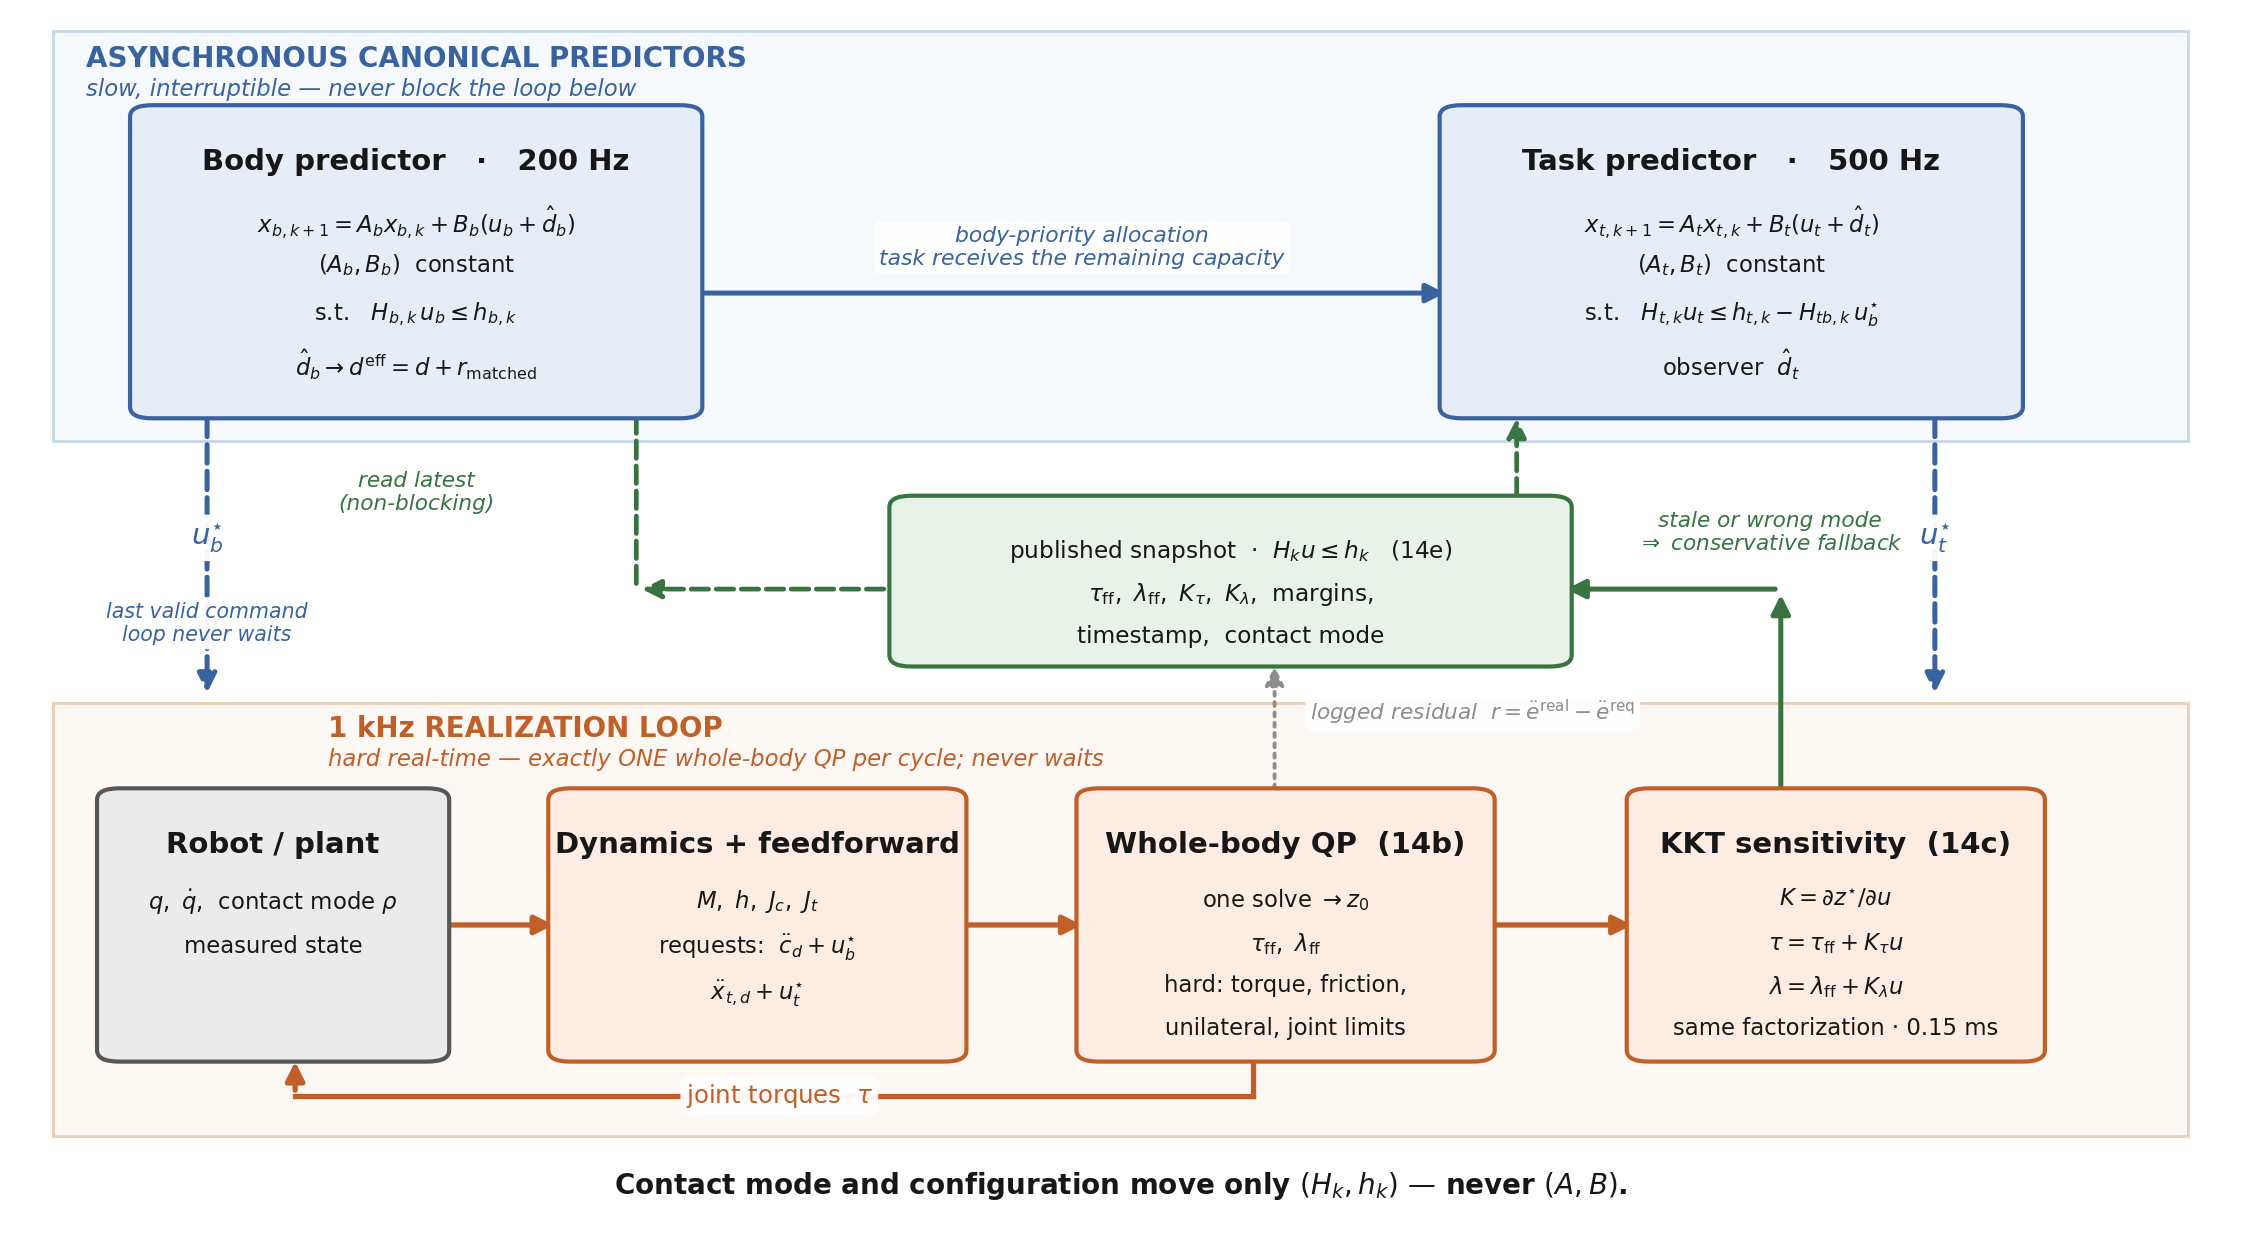
\includegraphics[width=0.98\textwidth]{figures/multirate_architecture.png}
\caption{The multirate interaction-dynamics architecture. One 1\,kHz realization loop (orange) solves a single whole-body QP per cycle and publishes an authority snapshot from one KKT solve; two asynchronous canonical predictors (blue) consume it and never block the loop. Contact mode and configuration move only the admissible set $(H_k,h_k)$, never the canonical pair $(A,B)$.}
\label{fig:arch}
\end{figure*}


\section{Related Work}\label{sec:related}

Centroidal and single-rigid-body MPC \cite{b2}, \cite{b3}, \cite{b8}, \cite{b13} predict CoM and body orientation while optimizing contact forces over a gait schedule, with horizon-wide treatment of friction, unilateral contact, and support geometry. The proposed body port instead predicts a normalized residual acceleration. At the current sample, the whole-body realizer maps the physical constraints into a conservative residual-command set; that set, or a mode-scheduled sequence of such sets, constrains the canonical predictor without adding contact forces to its decision vector.

Whole-body inverse dynamics and hierarchical QPs \cite{b4}, \cite{b5}, \cite{b7}, \cite{b9} enforce rigid contacts, task priorities, and actuator limits; they remain essential here as the instantaneous realizer that maps a desired body wrench and task acceleration to feasible generalized forces, not as another predictive model.

Operational-space impedance, admittance, and task-space MPC \cite{b6}, \cite{b11}, \cite{b12} regulate the end-effector port; their apparent inertia depends on configuration and support. Residual-acceleration coordinates remove this inertia from the prediction dynamics while retaining it in force recovery.

Learning-based pipelines increasingly \emph{generate} whole-body references: reinforcement-learning policies and human-demonstration retargeting engines produce rich, contact-consistent trajectories at a scale hand-authored planners cannot match. But a kinematic reference, however expressive, does not guarantee the motion is executable under real contact forces, actuator limits, and unexpected interaction; running it on hardware still needs a local, model-based layer that enforces constraints and supplies reactive compliance. The present framework is exactly that layer --- it takes a reference, hand-authored or learned, and provides the constraint-aware interaction-dynamics realization that turns kinematic intent into safe torque-level execution, rather than competing with the generator.

Closest in spirit is unified whole-body MPC for locomotion and manipulation \cite{b10}, which optimizes a single predictive whole-body model. We differ in the prediction--realization split: only the two normalized interaction dynamics are predicted, while the full contact-constrained dynamics act at the current sample as a feasibility projection, not a second predictive model. The normalized model, offset-free regulation, stability conditions, and impedance interpretation belong to \cite{b1}; the standard centroidal model \cite{b8}, \cite{b17}, whole-body inverse dynamics \cite{b9}, and the integrating-disturbance observer \cite{b16} are prior tools. This paper contributes their floating-base integration, anticipatory coupling, constraint realization, and evaluation on a Unitree G1 in MuJoCo \cite{b15}.

\section{Floating-Base Interaction Dynamics}\label{sec:dynamics}

Let

\[
q=[q_b^\top,q_j^\top]^\top,\qquad
M(q)\ddot q+h(q,\dot q)=S^\top\tau+J_c^\top\lambda+J_t^\top F_h,
\tag{2}
\]

where \(q_b\) is the floating-base coordinate, \(q_j\) contains actuated joints, \(\lambda\) stacks contact wrenches, and \(F_h\) is an external task wrench. Rigid active contacts satisfy

\[
J_c\ddot q+\dot J_c\dot q=0.
\tag{3}
\]

The controller uses two controlled ports. The body port is defined by CoM position and body-orientation errors --- the orientation channel regulated in centroidal angular-momentum coordinates (Section IV), with a desired attitude entering only through an outer loop --- and the task port is defined by Cartesian end-effector tracking error. The active contact mode \(\rho\) changes the contact Jacobian and feasible wrench set. Following \cite{b1}, it does not change the normalized prediction pair used below. This invariance is the organizing idea of the paper, which we state once and then use throughout.

\textbf{Definition 1 (interaction-dynamics representation, under exact feedforward normalization).} An \emph{interaction-dynamics representation} of a controlled port consists of: (i) a canonical requested model \(\ddot e=u+d\) whose exact-ZOH state-transition pair \((A,B)\) is independent of the robot's mechanics; (ii) a realization-informed admissible set \(\widehat{\mathcal U}_k\) supplied at every MPC update from the current robot state, reference feedforward, contact mode, and physical constraints; and (iii) an instantaneous recovery map that realizes the selected command and reports the residual \(r=\ddot e^{\rm real}-(u+d)\). Robot mechanics therefore do not enter \((A,B)\), but they do enter the input geometry \(\widehat{\mathcal U}_k\) and recovery map.

The qualifier is essential, and we make its hypotheses explicit.

\textbf{Assumption 1 (exact feedforward normalization).} A controlled port has physical coordinate \(x\) with tracking error \(e = x - x_d\), and constrained dynamics \(M_p(q,\rho)\ddot x + \mu_p(q,\dot q,\rho) = F_p^{\rm act} + F_p^{\rm ext}\), where the \emph{interaction inertia} \(M_p\) is invertible and well-conditioned on the operating set. The commanded actuation cancels the bias and injects the desired-trajectory plus residual acceleration, \(F_p^{\rm act} = \mu_p + M_p(\ddot x_d + u) + \delta\), and the recovery map \(u \mapsto F_p^{\rm act}\) is affine on each active-constraint cell.

\textbf{Theorem 1 (canonical dynamics invariance).} Under Assumption 1, every such port admits the normalized realized model \(\ddot e=u+d+r\), with residual-acceleration input \(u\), interaction disturbance \(d=M_p^{-1}F_p^{\rm ext}\), and realization residual \(r=M_p^{-1}\delta\). The exact-ZOH pair \((A,B)\) of the requested integrator chain is independent of \(M_p\), \(\mu_p\), and contact mode \(\rho\). These quantities may change the admissible input set \(\widehat{\mathcal U}_k\) and recovery map at every update, but they do not change the canonical state-transition matrices. Hence a contact transition is constraint switching, not dynamics switching, in the requested coordinates.

\emph{Proof sketch.} Substituting the feedforward of Assumption 1 into the constrained dynamics cancels \(\mu_p\), leaving \(M_p\ddot x = M_p(\ddot x_d + u) + F_p^{\rm ext} + \delta\); subtracting \(M_p\ddot x_d\) and left-multiplying by \(M_p^{-1}\) gives \(\ddot e = \ddot x - \ddot x_d = u + d + r\). The map from \(u\) to \(\ddot e\) is the identity, so the sampled predictor is the integrator ZOH pair, which contains no entry of \(M_p\), \(\mu_p\), or \(\rho\). \(\square\)

\textbf{Remark (dynamics-invariant does not mean physics-blind).} Under actuation redundancy the recovery map is generally non-unique: different QP weightings, task priorities, and contact-force allocations produce different local authority sets and residuals, while sharing the same \((A,B)\). The invariant object is the requested dynamics, not the available control authority. Upstream planners may reuse the canonical transition pair, but they must accept the current admissible geometry supplied by the robot-specific realizer.

Intuitively, the representation behaves like a stable software interface with a capability query. The transition contract \(\ddot e=u+d\) does not change across robots or contacts, but the realizer reports which \(u\) values it can currently honor. As shown in Fig. 2, state/reference/contact data produce \(\widehat{\mathcal U}_k\), the constrained predictor selects \(u\in\widehat{\mathcal U}_k\), the realizer executes it, the residual \(r\) closes the realization account, and the Kalman observer estimates \(d\). Different robots therefore share one transition interface while exposing different current authority.

\begin{figure}[!t]
\centering
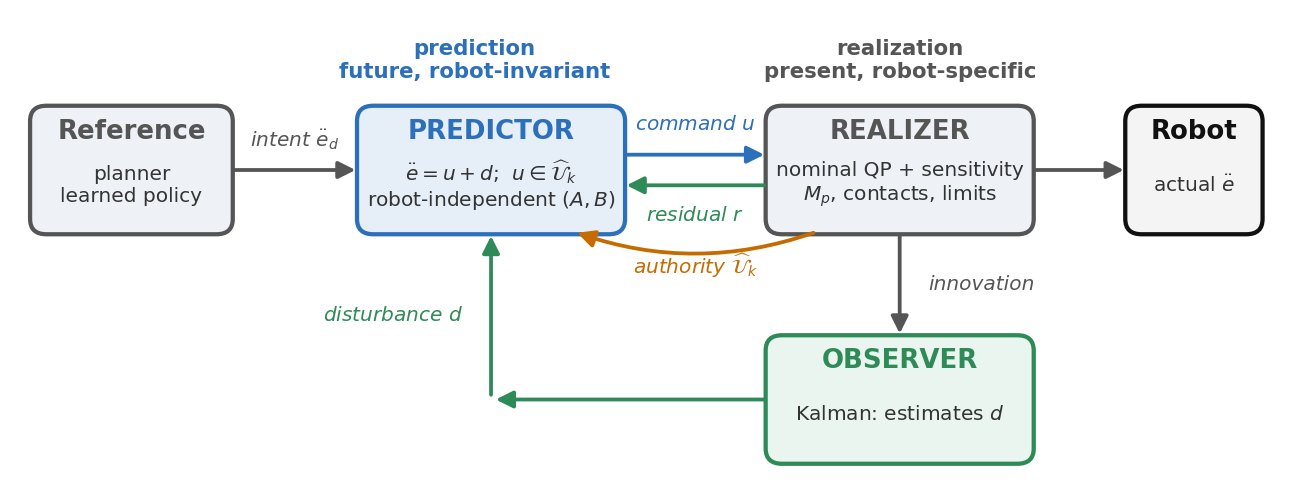
\includegraphics[width=\columnwidth]{figures/prediction_realization_concept.png}
\caption{Prediction--realization interface.}
\label{fig:concept}
\end{figure}


\section{Body Interaction Port}\label{sec:body}

\subsection{Centroidal Normalization}

Let \(c\) be the CoM, \(m\) the robot mass, \(f_i\) the force at active contact \(i\), and \(g\) the signed gravitational-acceleration vector (so \(mg\) is the weight). With lumped disturbance \(w_c\),

\[
m\ddot c=\sum_{i\in\mathcal C_\rho}f_i+mg+w_c.
\tag{4}
\]

For \(e_c=c-c_d\), define the desired resultant

\[
F_c^{\rm des}=m(\ddot c_d-g)+m u_c.
\tag{5}
\]

When the recovered contact forces satisfy \(\sum_i f_i=F_c^{\rm des}\),

\[
\ddot e_c=u_c+d_c,\qquad d_c=m^{-1}w_c.
\tag{6}
\]

The rotational channel is expressed directly in centroidal \textbf{angular-momentum} coordinates, which avoids identifying the locked-inertia angular velocity with a rigid-body attitude rate. Let \(k_G=A_G(q)\dot q\) be the centroidal angular momentum, with \(A_G\) the angular block of the centroidal momentum matrix, and let \(M_c\) be the net contact moment about the CoM. Then

\[
\dot k_G=M_c+w_\theta,
\tag{7}
\]

where \(w_\theta\) lumps unmodeled moments. For the angular-momentum error \(e_h=k_G-k_{G,d}\), define the desired net moment

\[
M_c^{\rm des}=\dot k_{G,d}+u_\theta.
\tag{8}
\]

When the recovered contacts realize \(M_c=M_c^{\rm des}\),

\[
\dot e_h=u_\theta+d_\theta,\qquad d_\theta=w_\theta,
\tag{9}
\]

a \textbf{first-order} integrator. Unlike an attitude parametrization, (9) is exact under exact moment recovery: no locked-inertia-to-attitude approximation is introduced. When a desired attitude is required, it is supplied through the reference \(k_{G,d}\) by an outer regulator (for example \(k_{G,d}=-K_\theta\,\log(RR_d^\top)^\vee\)); the local validity of that attitude map is then a property of the outer loop, not of the port dynamics. The two body channels therefore differ in order --- a second-order integrator on the CoM error and a first-order integrator on the angular-momentum error --- rather than being forced into a common attitude double integrator.

Crucially, neither the requested translational relation (6) nor the requested rotational relation (9) is the true plant: the recovered resultant force and net moment are realized by the whole-body layer only up to a \textbf{realization residual} (Section VI), which is retained explicitly rather than folded silently into \(d\). Writing that residual as \(r_b=[r_c^\top,r_h^\top]^\top\), the physically realized body port obeys

\[
\ddot e_c=u_c+d_c+r_c,\qquad
\dot e_h=u_\theta+d_\theta+r_h,
\tag{6$'$}
\]

with \(r_b=0\) exactly when the requested centroidal wrench and moment are feasibly recovered. Stacking the second-order CoM channel and the first-order angular-momentum channel,

\[
x_b=[e_c^\top,\dot e_c^\top,e_h^\top]^\top,\quad
u_b=[u_c^\top,u_\theta^\top]^\top,\quad
d_b=[d_c^\top,d_\theta^\top]^\top,
\]

and applying the exact-ZOH construction of \cite{b1} to the requested model at period \(T_b\) --- with the inputs \(u_b\), \(d_b\), and \(r_b\) held constant over each sampling interval (the standard zero-order-hold hypothesis) --- gives

\[
x_{b,k+1}=A_bx_{b,k}+B_b(u_{b,k}+d_{b,k}+r_{b,k}),
\tag{10}
\]

\[
A_b=
\begin{bmatrix}I_3&T_bI_3&0\\0&I_3&0\\0&0&I_3\end{bmatrix},
\qquad
B_b=
\begin{bmatrix}
\tfrac12T_b^2I_3&0\\
T_bI_3&0\\
0&T_bI_3
\end{bmatrix}.
\tag{11}
\]

The pair \((A_b,B_b)\) is constant; mass, centroidal inertia, contact locations, and contact mode appear only in wrench recovery and constraints.

\textbf{Proposition 1 (canonical body-port representation; Theorem 1 for the body port).} For a fixed active contact mode, the \emph{requested} body-port dynamics are the canonical model (10) with the constant exact-ZOH pair (11): a double integrator on the CoM error and a first-order integrator on the centroidal angular-momentum error. The translational channel follows exactly from centroidal force balance (4)--(6); the rotational channel follows exactly from centroidal angular-momentum balance (7)--(9), with no attitude approximation. Mass, centroidal inertia, contact locations, friction, and center-of-pressure limits enter only the recovery map and the feasible input set, not \((A_b,B_b)\). The realized body port equals the requested model up to the realization residual \(r_b\) of Section VI, and coincides with it when \(r_b=0\).

\textbf{Proof.} Substituting the recovered resultant (5) into (4) gives (6); substituting the recovered moment (8) into (7) gives (9). Stacking yields a block-diagonal continuous-time generator (double integrator \(\oplus\) first-order integrator) whose exact zero-order hold is (11) --- the first-order block \(\dot e_h=u_\theta+d_\theta\) discretizes exactly as \(e_{h,k+1}=e_{h,k}+T_b(u_{\theta,k}+d_{\theta,k})\). The quantities \(m\), \(A_G\), \(p_i\), \(\rho\) convert \(u_b\) into a centroidal wrench and contact forces through the recovery (12)--(15); the gap between requested and recovered wrench/moment is the residual \(r_b\) defined in Section VI. \(\square\)

\subsection{Contact-Wrench Recovery and MPC}

For stacked contact forces \(f=[f_1^\top,\ldots,f_{n_c}^\top]^\top\), define

\[
\mathcal G_\rho(c,p_i)f=
\begin{bmatrix}
\sum_i f_i\\
\sum_i(p_i-c)\times f_i
\end{bmatrix}.
\tag{12}
\]

The desired centroidal wrench is

\[
W_b^{\rm des}(u_b)=
\begin{bmatrix}
m(\ddot c_d-g)+mu_c\\
\dot k_{G,d}+u_\theta
\end{bmatrix}.
\tag{13}
\]

Recovery enforces

\[
\mathcal G_\rho f=W_b^{\rm des}(u_b)+s_W,
\tag{14}
\]

where \(s_W\) is a penalized wrench residual that is zero under exact recovery and may become nonzero under infeasibility or weighted task tradeoffs (hard recovery would require \(s_W=0\) as a constraint or lexicographic priority). This residual maps to the body-port acceleration residual of (6\('\)): its force part gives \(r_c=m^{-1}s_W^{\rm (force)}\) and its moment part \(r_h=s_W^{\rm (moment)}\). We keep \(r_b\) explicit rather than folding it into \(d_b\) --- \(d_b\) is the external/model disturbance the observer cancels, \(r_b\) a physical-infeasibility residual no input can remove --- so (6), (9), and (10) are exact when \(r_b=0\) and hold with a logged acceleration residual otherwise. Under a scheduled contact sequence the recovery map \(\mathcal G_{\rho_j}\) is re-formed per mode while \((A_b,B_b)\) stay unchanged.

Under the prediction--realization separation the body MPC predicts only the canonical state transition; it does not duplicate \(M\), \(J_c\), contact forces, or joint torques across the horizon. It is nevertheless constrained by the current physical capability, and that constraint is obtained from the whole-body QP the realizer is \emph{already solving} --- not from a second optimization.

\textbf{The solved form of the realizer.} Eliminating the slacks \(s_W,s_t\) of (22) against their quadratic penalties turns the realizer into the weighted problem actually solved,
\begin{equation}
\min_{z}\ \tfrac12 z^\top P z+\big(q_0+Q_u\,u\big)^\top z
\quad\text{s.t.}\quad Ez=e,\qquad Cz\le c,
\tag{14b}
\end{equation}
with \(z=[\ddot q^\top,\tau^\top,\lambda^\top]^\top\), \(Ez=e\) the rigid-body dynamics and rigid-contact rows, and \(Cz\le c\) the actuator bounds, friction pyramid, unilateral-force and one-step joint limits --- all of which remain \textbf{hard}. The stacked residual command \(u=[u_b^\top,u_t^\top]^\top\) enters (14b) only through the \emph{linear} term, via the CoM-acceleration, centroidal-wrench and end-effector-acceleration targets; the Hessian \(P\) does not depend on \(u\). This is the structural fact the rest of the section rests on, and it is a property of the eliminated form (14b), not of the slack form (22).

\textbf{Authority from one KKT solve.} Let \(\mathcal A_k\) index the rows of \(Cz\le c\) active at the current solution \(z_0=z_k^\star(0)\) --- identified from the solver's duals, a row being active when it sits at its bound and its multiplier exceeds \(\varepsilon_\lambda\) --- and let \(C_{\mathcal A_k}\) stack those rows together with the equality rows \(E\), which are always active. On the \emph{critical region} where \(\mathcal A_k\) is unchanged, the solution of (14b) is affine in \(u\) and its Jacobian solves
\begin{equation}
\begin{bmatrix}P & C_{\mathcal A_k}^{\!\top}\\ C_{\mathcal A_k} & 0\end{bmatrix}
\begin{bmatrix}K\\ \ast\end{bmatrix}=\begin{bmatrix}-\,Q_u\\ 0\end{bmatrix},
\qquad z_k^\star(u)\approx z_0+Ku .
\tag{14c}
\end{equation}
The nominal whole-body QP supplies \(z_0\) --- hence the feedforward \(\tau_{\rm ff},\lambda_{\rm ff}\) --- and (14c) supplies only the sensitivity \(K\); partitioning it gives the input maps, so that
\begin{equation}
\tau=\tau_{\rm ff}+K_\tau u,\qquad \lambda=\lambda_{\rm ff}+K_\lambda u .
\tag{14d}
\end{equation}

\textbf{Mapped constraints.} Substituting (14d) into the physical limits the realizer already enforces, and into the realization-tolerance test \(\lVert r_k(u)\rVert_\infty\le\epsilon_r\) linearized about the same cell, yields
\begin{equation}
\widehat{\mathcal U}_k=\{u:\ H_k u\le h_k\}.
\tag{14e}
\end{equation}
Three properties must be stated plainly. \emph{(i)} The tolerance rows are not optional: a command can satisfy every actuator and contact limit and still fail to be realized, because the realizer trades the request against its other objectives. \emph{(ii)} A row with \(h_{k,i}<0\) means the nominal solution already sits past that \textbf{margin} --- never past a true limit, since (14b) enforces the true limits as hard constraints --- and is clamped at zero, which keeps \(u=0\) admissible. Soundness therefore rests on the realizer's hard constraints, not on the construction of (14e); \(\widehat{\mathcal U}_k\) is an inner \emph{model}, not a certificate. \emph{(iii)} The affine map (14c) is exact only on the current critical region: once a new constraint activates the true QP redistributes and the map bends. The resulting conservatism is measured, not assumed (Section~X-E), and the realizer remains the final hard layer.

\textbf{Beyond one cell: piecewise-affine continuation.} The set (14e) is, in essence, the \emph{critical region} of the active set \(\mathcal A_k\) --- the region on which no new constraint activates. But an active-set change is not a failure of realization: when a contact force saturates, another takes over and the request is still met. The true feasible set therefore spans several critical regions, and (14e) refuses most of it.

The remedy uses no new machinery. Along a ray \(u=t\,e\), the solution is affine until one of exactly two events occurs: an inactive row of \(Cz\le c\) reaches its bound (a constraint \textbf{enters} \(\mathcal A_k\)), or an active row's multiplier reaches zero (a constraint \textbf{leaves}). Both are available in closed form from the KKT system (14c), whose primal block gives \(\mathrm dz/\mathrm du\) and whose \emph{dual} block gives \(\mathrm d\nu/\mathrm du\); the first event is the smaller of the two breakpoints. There \(\mathcal A_k\) is updated, (14c) is re-solved, and the walk continues. Because the realization residual is affine on each region, the tolerance crossing is exact, and \emph{that} crossing is the authority boundary. The walk costs one KKT solve per region traversed and --- the essential point --- \textbf{no whole-body QP solves at all}. Section~X-E shows it recovers the exact feasible set.

Because \(H_k,h_k\) come from a single KKT solve on a factorization the realizer already possesses, the set is refreshed inside the 1\,kHz realization loop at a cost of \(\approx0.15\) ms --- as against \(\approx154\) ms for the exact multi-query search, retained only as an offline oracle (Section~X-E). For split body/task MPCs a \textbf{body-priority allocation} is used: the body slice is computed with the task request at nominal, and the task port receives the remaining capacity \(H_tu_t\le h_t-H_{tb}u_b^\star\) from the same joint sensitivity, at no extra QP or KKT solve.

The controller interface permits an authority refresh at every MPC update. The resulting set is frozen over the short horizon, so the transition matrices $(A_b,B_b)$ and the predictor's condensed \emph{cost} Hessian $\Psi$ --- the quadratic form of the lifted problem (15), which depends only on $A_b,B_b,Q_b,R_b$ and the horizon, never on the robot --- remain constant, while only the constraint rows change. Note that $\Psi$ is a \emph{cost} matrix and must not be confused with the \emph{constraint} matrix $H_k$ of (14e); the whole point is that $\Psi$ is invariant while $H_k$ is not. For a known contact switch inside the horizon, the scheduled formulation uses mode-dependent sets; a transition window may use \(\widehat{\mathcal U}_{\rm tr}=\widehat{\mathcal U}_{\rm DS}\cap\widehat{\mathcal U}_{\rm SS}\). This intersection reduces incompatible requests but does not by itself prove recursive feasibility.

The body MPC is therefore

\[
\begin{aligned}
\min_{U_b}\quad&
\sum_{j=0}^{N_b-1}
\left(
\|x_{b,j}\|_{Q_b}^2+
\|u_{b,j}+\hat d_{b,k}\|_{R_b}^2
\right)
+\|x_{b,N_b}\|_{S_b}^2\\
\text{s.t.}\quad&
x_{b,j+1}=A_bx_{b,j}+B_b(u_{b,j}+\hat d_{b,k}),\\
&u_{b,j}\in\widehat{\mathcal U}_{b,k}.
\end{aligned}
\tag{15}
\]

No robot-specific quantity enters the state-transition matrices or quadratic cost. Current mechanics enter only through \(\widehat{\mathcal U}_{b,k}\) and through instantaneous recovery and residual after the first command is applied. The set is recomputed at 1 kHz by the realizer and consumed asynchronously by the predictor, which never blocks on it; a stale or mode-mismatched set is replaced by a conservative fallback. Contact transitions therefore schedule admissible geometry while leaving \((A_b,B_b)\) unchanged.

\textbf{Why the realization residual does not appear in (15).} The realized plants (10) and (20) carry \(r\); the predictors (15) and its task analogue do not. This is deliberate, and it is the point of the construction.

First, \(r\) is not an exogenous signal that could be predicted or cancelled: it is a \emph{function of the decision variable}, \(r=r(u)\), zero while the request lies in the realizable set and growing once it leaves it. Adding it to the prediction model as an additive input would be a category error.

Second, the constraint \(u_{b,j}\in\widehat{\mathcal U}_{b,k}\) \textbf{is} the predictor's representation of \(r\): the admissible set is precisely the set on which the realizer can honor the request, i.e.\ on which \(r\approx0\). Constraining the command to it \emph{and} carrying an additive \(r\) term would count the same physics twice.

Third, the predictor cannot know \(r\) over the horizon in any case: the realizer reports it only after the command has been executed.

What remains is the part of \(r\) the constraint fails to prevent --- because the set is a local model, because it is frozen over the horizon, or because the request was infeasible from the start. That part splits in two. Its matched, slowly varying component is indistinguishable from a disturbance in the measured error and is absorbed by the observer of Section~VIII, whose estimate converges not to \(d\) but to an \textbf{effective} disturbance \(d^{\rm eff}=d+r_{\rm matched}\); the predictor cancels it without ever attributing it. The remaining unmatched component is what no feasible input can remove, and it is bounded --- not modelled --- by Proposition~6. Accordingly (15) predicts the \emph{requested} dynamics and confines every consequence of physical infeasibility to the constraint set and the logged residual.

The input-centered penalty is essential: for a constant estimated disturbance the cancelling equilibrium is \(u_b=-\hat d_b\), so penalizing \(\|u_b+\hat d_b\|\) rather than \(\|u_b\|\) avoids reintroducing a steady-state offset.

\section{Task Interaction Port}\label{sec:task}

The task port is not derived from a fixed-base arm model. In (2), \(M(q)\) is the full floating-base mass matrix, including the unactuated base and all actuated joints, and \(J_{c,\rho}\) is the active whole-body contact Jacobian. Using the contact-consistent inverse associated with mode \(\rho\),

\[
\bar M_\rho^{-1}
=M^{-1}-M^{-1}J_{c,\rho}^\top
(J_{c,\rho}M^{-1}J_{c,\rho}^\top)^{-1}
J_{c,\rho}M^{-1},
\tag{16}
\]

the task inertia is

\[
\Lambda_t=(J_t\bar M_\rho^{-1}J_t^\top)^{-1}.
\tag{17}
\]

Thus \(\Lambda_t\) already contains the floating-base, stance-contact, and arm--body inertial coupling of the full constrained system; it does not assume the arm is dynamically isolated from the base, only expresses the realized task acceleration in residual-acceleration coordinates after the current contacts are imposed. Predictable base reactions are handled by the coupled body-port preview (Section VII); unmodeled coupling and recovery error go into \(d_t\) and the realization residuals of (22).

Projecting the constrained rigid-body dynamics into the task coordinates gives the contact-consistent task-space dynamics

\[
\Lambda_t\,\ddot x_t+\mu_{t,\rho}=F_t^{\rm act}+F_h+r_{t,\rm dyn},
\tag{17b}
\]

where \(\mu_{t,\rho}=\bar J_t^\top h-\Lambda_t\dot J_t\dot q\) collects Coriolis, centrifugal, and gravity terms, \(F_t^{\rm act}\) is the task-space wrench \emph{actually} produced by the joint torques, \(F_h\) is the external task wrench, and \(r_{t,\rm dyn}\) lumps contact-consistency and higher-priority null-space couplings. For \(e_t=x_t-x_{t,d}\), the controller \textbf{requests} the wrench

\[
F_t^{\rm cmd}=F_{t,\rm ff}+\Lambda_tu_t,\qquad
F_{t,\rm ff}=\Lambda_t\ddot x_{t,d}+\mu_{t,\rho},
\tag{18}
\]

equivalently the acceleration request \(\ddot x_t^{\rm req}=\ddot x_{t,d}+u_t\). Let \(\ddot x_t^{\rm real}\) be the acceleration the whole-body realizer actually imposes, and define the \textbf{realization residual}

\[
r_t=\ddot x_t^{\rm real}-\ddot x_t^{\rm req}.
\tag{18b}
\]

Substituting (18) into (17b): when the requested wrench is realized exactly (\(F_t^{\rm act}=F_t^{\rm cmd}\), \(r_t=0\)) the nominal acceleration cancels and \(\ddot e_t=u_t+\Lambda_t^{-1}F_h+d_{\rm model}\). In general the realized task port is

\[
\ddot e_t=u_t+d_{h,t}+r_t,\qquad
d_{h,t}=\Lambda_t^{-1}F_h+d_{\rm model},
\tag{19}
\]

with \(d_{h,t}\) the observer-cancelled external/model disturbance and \(r_t\) the physical-infeasibility residual (kept distinct, as for the body port). Exactly as for the body port (10), the \emph{realized} task port discretizes by exact ZOH as

\[
x_{t,k+1}=A_tx_{t,k}+B_t(u_{t,k}+d_{h,t,k}+r_{t,k}),
\tag{20}
\]

with

\[
A_t=\begin{bmatrix}I_3&T_tI_3\\0&I_3\end{bmatrix},
\qquad
B_t=\begin{bmatrix}\tfrac12T_t^2I_3\\T_tI_3\end{bmatrix},
\tag{20b}
\]

the canonical three-dimensional exact-ZOH double-integrator pair.

\textbf{Proposition 2 (contact-consistent task port).} For a fixed active contact mode with \(J_{c,\rho}M^{-1}J_{c,\rho}^\top\) and \(J_t\bar M_\rho^{-1}J_t^\top\) nonsingular on the operating set, the \emph{requested} end-effector port is the canonical model (20) with a constant exact-ZOH pair; configuration and contact mode enter through \(\Lambda_t\), the feedforward \(\mu_{t,\rho}\), and the feasible set, not through \((A_t,B_t)\). The realized port equals the requested model up to \(r_t\), and coincides with it when \(r_t=0\).

\textbf{Proof.} The constrained inverse (16), formed from the full floating-base mass matrix, restricts admissible accelerations to directions compatible with the active rigid contacts, giving the contact-consistent apparent inertia \(\Lambda_t\) (17). Substituting the commanded wrench (18) into the constrained task dynamics (17b) cancels the nominal terms and leaves (19); the exact ZOH of the requested part is (20). The gap \(r_t\) between requested and realized task acceleration is the realizer residual \(s_t\) of (22). \(\square\)

Like the body port, the task MPC retains the canonical transition pair and minimizes \(\sum_j\!\big(\|x_{t,j}\|_{Q_t}^2+\|u_{t,j}+\hat d_{t,k}\|_{R_t}^2\big)+\|x_{t,N_t}\|_{S_t}^2\). Its constraint is not a fixed end-effector acceleration box. The same joint KKT sensitivity (14c) that produced the body maps also produces the task maps \(K_{\tau,t},K_{\lambda,t}\), at no extra solve. Under the body-priority allocation the body command \(u_{b,k}^\star\) is committed first and consumes part of the shared actuator and contact budget; the task port then receives what remains,
\begin{equation}
\widehat{\mathcal U}_{t,k}=\{u_t:\ H_{t,k}\,u_t\le h_{t,k}-H_{tb,k}\,u_{b,k}^\star\}.
\tag{21}
\end{equation}
The rows of (21) are the actuator, friction, unilateral-force and task-tolerance limits mapped through \(\tau=\tau_{\rm ff}+K_{\tau,b}u_b^\star+K_{\tau,t}u_t\) and the corresponding contact-force map, so they express the \emph{remaining} residual authority after gravity, desired motion, balance and the committed body request have consumed shared capability. The allocation is a policy, not an equivalence to a joint body--task optimization. Near a task singularity or torque boundary the set contracts; when the nominal task residual already exceeds the task tolerance the set is empty, and the predictor must fall back rather than issue a command the realizer cannot honor.

\section{Whole-Body Interaction Realizer}\label{sec:realizer}

The two MPCs output a body request (a centroidal wrench \(W_b^{\rm des}\), realized by the contact forces) and a task request (the end-effector acceleration \(\ddot x_{t,d}+u_t^\star\), realized by the joint torques). Under exact, unconstrained recovery this acceleration and the commanded wrench \(F_t^{\rm cmd}\) correspond through \(\Lambda_t\), but the correspondence breaks once torque saturation, friction/CoP limits, or a higher-priority balance task force the realizer to trade the request against constraints and report the shortfall as \(s_t=r_t\); imposing the task as an acceleration and exposing \(s_t\) is the honest form, while the body request stays a wrench because that is what the unilateral, friction, and CoP constraints act on. This layer predicts no future states --- it is not an MPC but an instantaneous projection of both requests onto the generalized accelerations, contact wrenches, and joint torques satisfying the floating-base dynamics and constraints.

Let \(S_j\) select the actuated joint coordinates from \(q\), and let \(\tau_{\rm ref}\) be a nominal torque used only for regularization, such as the previous command or a gravity-compensating inverse-dynamics torque. With polyhedral friction pyramids, the whole-body interaction realizer is the convex instantaneous inverse-dynamics QP

\[
\begin{aligned}
\min_{\ddot q,\tau,\lambda,s_W,s_t}\quad&
\|s_W\|_{W_b}^2
+\|s_t\|_{W_t}^2
+\|\tau-\tau_{\rm ref}\|_{W_\tau}^2\\
\text{s.t.}\quad&
M\ddot q+h=S^\top\tau+J_c^\top\lambda+J_t^\top F_h,\\
&J_c\ddot q+\dot J_c\dot q=0,\\
&\mathcal G_\rho\lambda=W_b^{\rm des}+s_W,\\
&J_t\ddot q+\dot J_t\dot q=\ddot x_{t,d}+u_t^\star+s_t,\\
&\lambda\in\mathcal F_\rho,\quad
\tau_{\min}\le\tau\le\tau_{\max},\\
&q_j^+=S_j(q+\Delta t\dot q+\tfrac12\Delta t^2\ddot q),\\
&q_{j,\min}+\epsilon\le q_j^+\le q_{j,\max}-\epsilon.
\end{aligned}
\tag{22}
\]

The external wrench \(F_h\) in the dynamics row is a known constant, not a decision variable, and is used in one of two \emph{mutually exclusive} modes so the same wrench is never compensated twice: (i) \emph{measured-wrench feedforward} --- the sensed \(F_h\) is inserted into the dynamics equality and its contribution is removed from the task disturbance state, so the observer estimates only the residual; or (ii) \emph{observer-only rejection} --- \(F_h\) is set to zero in the dynamics equality and the residual-acceleration input \(u_t\) cancels the estimated disturbance \(\hat d_t\). Inserting \(\Lambda_t\hat d_t\) as a known physical wrench \emph{and} cancelling it through \(u_t\) would double-count and is not done. The decision variables are \(\ddot q\), \(\tau\), the contact wrench \(\lambda\), and two realization slacks: \(s_W=\mathcal G_\rho\lambda-W_b^{\rm des}\), a six-dimensional \emph{wrench} residual (N and N·m --- the body-port slack of (14)), and \(s_t=(J_t\ddot q+\dot J_t\dot q)-(\ddot x_{t,d}+u_t^\star)\), a task-\emph{acceleration} residual. Both are \emph{realized minus requested}. Because \(s_W\) is a wrench while the body residual \(r_b\) of (6\('\)) is an acceleration, they are related by \(r_b=\mathcal D_b\,s_W\) with \(\mathcal D_b=\operatorname{diag}(m^{-1}I_3,I_3)\) (force part \(r_c=m^{-1}s_W^{\rm (force)}\), moment part \(r_h=s_W^{\rm (moment)}\), matching (14)); the task residual matches directly, \(s_t=r_t\). The first two equalities enforce rigid-body dynamics and contact consistency; the joint-limit row's \(\frac12\Delta t^2\ddot q\) term is what makes the one-step check depend on the decision variable rather than only the current state.

With a friction-pyramid approximation \(\mathcal F_\rho\) is polyhedral and (22) is a convex QP solvable by operator splitting \cite{b14}; exact Coulomb cones make it a second-order cone program. Balance can be made hard (\(s_W=0\)) or soft (large \(W_b\)), and task tracking is softened through \(s_t\) when the two requests conflict.

The realizer has two current-sample roles, and performs \textbf{one} QP solve to serve both. Solving (14b) yields the torques applied this sample and the nominal feedforward \(z_0=(\ddot q_0,\tau_{\rm ff},\lambda_{\rm ff})\); one KKT sensitivity (14c) on the same factorization then yields the input maps, and hence the admissible set (14e) published to the predictors. The realizer never runs a second optimization to answer the capability query. Having executed the first stacked request it reports

\[
u_k^{\rm req},\qquad
u_k^{\rm real},\qquad
r_k=u_k^{\rm real}-u_k^{\rm req},
\tag{22b}
\]

together with nominal torque/contact wrench, minimum torque/friction/CoP/joint margins, authority-set center and width, active constraint class, MPC-bound activation, final actuator clipping, and QP fallback. These signals distinguish three different events: the predictor reaching its admissible boundary, the realizer trading the request through \(s_W\) or \(s_t\), and a final numerical safety clip. They must not be reported as the same saturation event.

The authority query uses only current measured/estimated state and known references; it does not read future disturbance realizations. For a scheduled contact transition, future mode geometry may be supplied by the contact plan, but state-dependent queries must still be refreshed. The instantaneous realizer remains the final hard safety layer because a sampled box can be invalidated by inter-sample state motion, estimation error, and unmodeled contact.

\section{External-Wrench and Internal-Momentum Preview}\label{sec:preview}

The split controller solves the body MPC (15) and the task MPC independently; whatever the arm does reaches the body port only after it is observed, and is rejected reactively through \(d_b\). The coupled controller instead previews the \emph{planned} effect of the arm on the centroidal dynamics. Two physically distinct effects must be kept separate, because conflating them double-counts forces.

\textbf{External task wrench.} When the hand exchanges a real contact force with the environment --- pushing, carrying, leaning on a rail --- the environment reaction \(F_h^{\rm plan}\) (and moment \(M_h^{\rm plan}\)) enters the \emph{whole-robot} centroidal-momentum balance as a genuine external wrench, with known centroidal contribution

\[
W_{G,h}^{\rm ext}=
\begin{bmatrix}
F_h^{\rm plan}\\
(x_h-c)\times F_h^{\rm plan}+M_h^{\rm plan}
\end{bmatrix}.
\tag{23}
\]

The body port previews it by adding \(-W_{G,h}^{\rm ext}\) to the desired centroidal wrench (13) over the horizon, so the contacts are pre-loaded before \(d_b\) has to build up.

\textbf{Internal arm motion.} A fast \emph{free-space} reach exerts no external force on the robot. The operational-space control wrench \(F_t^{\rm ctrl}=F_{t,\rm ff}+\Lambda_t u_t\) acts through joint torques and is \emph{internal}; it must \textbf{not} be inserted into the centroidal balance as an external \(-F_t^{\rm ctrl}\), because internal actuation cannot change the total centroidal momentum and doing so double-counts. The genuine base reaction is the rate of change of centroidal momentum carried by the arm. Partitioning the centroidal momentum matrix into base, leg, and arm columns in \(h_G=A_G(q)\dot q\), the planned arm motion contributes

\[
\dot h_{G,\rm arm}^{\rm plan}
=A_{G,\rm arm}(q)\,\ddot q_{\rm arm}^{\rm plan}
+\dot A_{G,\rm arm}(q,\dot q)\,\dot q_{\rm arm}^{\rm plan},
\tag{23b}
\]

Equation (23b) is the internal reaction that a \emph{split} body predictor would need to exchange with an independently realized arm plan. In the unified current-sample whole-body QP used here, however, the arm columns already appear in the total CoM Jacobian. Adding \(-\dot h_{G,\rm arm}^{\rm plan}\) again to the body request therefore double-counts the same internal motion. External wrench preview remains explicit because the environment wrench is not generated by those internal generalized accelerations. The evaluation therefore varies planned external hand load as part of the nominal feedforward in Experiment 2; it does not add a duplicate internal arm wrench to the body request.

A single stacked QP is possible when both horizons share a grid; a simpler alternative retains two QPs and passes the planned arm wrench/momentum sequence to the body port. No equivalence between weighted and strict lexicographic priority is assumed; hard balance constraints, soft task objectives, and the logged acceleration residuals define the actual priority.

\section{Kalman Estimation and Contact Events}\label{sec:kalman}

Following the integrating-disturbance principle for zero steady-state error under persistent disturbances \cite{b16}, and its instantiation in \cite{b1}, each normalized model is augmented by a constant disturbance state:

\[
\begin{bmatrix}x_{k+1}\\d_{k+1}\end{bmatrix}
=
\begin{bmatrix}A&B\\0&I\end{bmatrix}
\begin{bmatrix}x_k\\d_k\end{bmatrix}
+
\begin{bmatrix}B\\0\end{bmatrix}u_k
+
\begin{bmatrix}0\\I\end{bmatrix}w_k.
\tag{24}
\]

Here \(w_k\) drives the disturbance random walk; process noise acting directly on \(x_k\) would be modeled by a separate state-noise term. The observer sees only the port error, in which a matched realization residual is indistinguishable from an external disturbance; its estimate therefore converges to the \textbf{effective} disturbance \(d^{\rm eff}=d+r_{\rm matched}\) of Section~IV, and it neither needs nor attempts to separate the two. The body observer estimates a six-dimensional residual wrench acceleration; the task observer estimates a three-dimensional residual acceleration. Offset-free regulation requires detectability, estimator convergence for a constant disturbance, and feasibility of the cancelling input.

The feedforward and recovery terms require generalized velocity. On hardware, \(\dot q\) should not be obtained by raw encoder differencing inside the high-rate loop. The intended implementation uses filtered velocity estimates, for example a low-order Butterworth low-pass or an observer-based differentiator feeding the rigid-body model; the high observer/QP rate keeps the resulting phase lag non-critical for closed-loop stability, and the residual lag and noise are absorbed by the disturbance state and the realization residuals. This filtering is an implementation requirement, not a theoretical replacement for torque-level validation.

A contact event creates an innovation because the assumed recovery set no longer matches the plant. This motivates a detector based on normalized innovation statistics:

\[
\eta_k=\nu_k^\top S_k^{-1}\nu_k.
\tag{25}
\]

A mode change is declared only after \(\eta_k\) exceeds a calibrated threshold for \(n_d\) consecutive samples and a candidate contact is geometrically plausible. This is safer than claiming that the aggregate disturbance alone uniquely identifies a particular foot: without additional kinematic information, different external wrenches can be indistinguishable at the centroidal port.

\section{Relation to the Fixed-Base Theory}\label{sec:theory}

The normalized predictor, nominal offset-free regulation, and impedance interpretation are taken directly from \cite{b1} and are not re-proved here. The new issue is whether the current whole-body realizer can communicate useful measured authority without changing the canonical dynamics.

\textbf{Proposition 3 (local affine recovery).} Fix the current state, references and contact mode, and let \(z_0\) solve (14b) with active set \(\mathcal A_k\). Suppose the active constraint gradients \(C_{\mathcal A_k}\) have full row rank (LICQ), strict complementarity holds, and \(P\) is positive definite on the null space of \(C_{\mathcal A_k}\). Then on the \emph{critical region} of \(\mathcal A_k\) we have \(z_k^\star(u)=z_0+Ku\) exactly, with \(K\) the unique solution of (14c).

\textbf{Proof.} Under LICQ and strict complementarity the active set is locally constant, so (14b) reduces to an equality-constrained QP whose optimality conditions are the linear system (14c). Since \(u\) enters only the linear cost term \(Q_uu\) and \(P\) does not depend on \(u\), the right-hand side is affine in \(u\) and the solution map is affine with Jacobian \(K\). \(\square\)

\textbf{Proposition 4 (mapped physical constraints).} On the same critical region, the actuator, friction-pyramid and unilateral-force limits of (14b), together with the linearized realization-tolerance test, are equivalent to \(H_ku\le h_k\) under the maps (14d). Hence every \(u\in\widehat{\mathcal U}_k\) that remains inside the critical region is realized with componentwise residual at most \(\epsilon_r\).

\textbf{Proof.} Substitution of (14d) into the affine constraint rows and of \(z_0+Ku\) into the residual expression, using Proposition 3. \(\square\)

\textbf{Remark (what Proposition 4 does \emph{not} give).} The guarantee is conditional on remaining in the critical region, which the predictor cannot verify. Outside it the true QP changes active set and the map bends, so \(\widehat{\mathcal U}_k\) is an inner \emph{model}, not a certified inner approximation, and no false-positive-free claim follows by construction. What holds unconditionally comes from the realizer, not the map: because (14b) enforces the actuator and contact limits as hard constraints, \emph{no} command can drive the robot past a physical limit; an inadmissible command is paid for in realization residual, not in constraint violation. The conservatism of the map is therefore an empirical quantity, measured against an offline oracle in Section~X-E.

\textbf{Remark (constraint-feasible does not mean faithfully realized).} Satisfying every torque and contact limit does not imply \(r=0\). The realizer trades the request against balance, posture and regularization objectives, so a request can be physically feasible and still be served poorly --- which is why the tolerance rows appear in (14e), and why a task port whose objective is weighted too softly has a large nominal residual and an empty authority set (Section~X-G).

\textbf{Proposition 4b (exactness of the continuation).} Suppose that along the ray \(u=t\,e\) the QP (14b) satisfies LICQ and strict complementarity except at finitely many breakpoints, and that no two breakpoints coincide. Then the piecewise-affine walk of Section~IV-B reproduces \(z_k^\star(t\,e)\) exactly up to the tolerance crossing, and the returned boundary is the exact boundary of \(\{t:\lVert r_k(te)\rVert_\infty\le\epsilon_r\}\).

\textbf{Proof sketch.} By Proposition 3 the solution is affine on each critical region, so it suffices to locate the boundaries and continue across them. A boundary occurs exactly when an inactive row becomes active or an active multiplier vanishes; both are affine in \(t\) and solved in closed form from (14c). Updating \(\mathcal A_k\) at the first breakpoint and re-solving (14c) yields the affine piece on the adjacent region. The residual is affine on each piece, so its tolerance crossing is exact. \(\square\)

\textbf{Remark (what remains empirical).} Degeneracy, coincident breakpoints, and the inexactness of the solver's duals can corrupt the active-set identification and hence the walk; the guarantee assumes them away. The zero false-positive and false-negative rates of Section~X-E are evidence, not proof, and the realizer stays the hard layer regardless. The walk is also a \emph{ray} construction: independent axis boundaries need not have feasible Cartesian corners.

\textbf{Proposition 5 (conditional offset-free regulation).} Fix a contact mode and suppose the realization residual is \emph{constant and matched} on the operating cell, so that the effective disturbance \(d^{\rm eff}=d+r_{\rm matched}\) is constant. If the augmented observer is detectable and \(\hat d\to d^{\rm eff}\), and if the cancelling request \(u=-d^{\rm eff}\) lies in \(\widehat{\mathcal U}_k\), then the regulated port reaches zero steady-state error under the fixed-base result of \cite{b1} --- the residual is \emph{cancelled along with} the disturbance, so \(r=0\) is not required, only that \(r\) be matched and constant. Two failure modes remain, both observed in Section~X: an unmatched or state-dependent residual cannot be cancelled by any input and yields only bounded regulation (Proposition~6); and when \(-d^{\rm eff}\) lies outside the admissible set --- as it does when the disturbance exceeds the port's authority --- no offset claim is made and the port saturates.

\textbf{Assumption 2 (nominal ISS).} The nominal requested-model closed loop of \cite{b1} --- the predictor \(\ddot e=u+d\) under the offset-free feedback of Section VIII --- is input-to-state stable with respect to its disturbance input.

\textbf{Proposition 6 (bounded authority mismatch).} Suppose Assumption 2 holds and that critical-region exit, snapshot staleness or inter-sample state motion leave a uniformly bounded realization residual, \(\sup_k\|r_k\|\le\varepsilon\). Then the realized augmented error state is ultimately bounded by the nominal class-\(\mathcal{KL}\) transient plus a class-\(\mathcal K\) gain on \(\varepsilon\). This does not certify \(\varepsilon\); it states how an authority mismatch propagates once the realizer has logged it.

\textbf{Imperfect feedforward on a floating base.} The exact-cancellation premise of Assumption 1 is never met exactly on the robot: arm--base reaction, configuration-dependent bias, and velocity-estimate error all leave a feedforward mismatch. This mismatch splits along the same \(d\)/\(r\) line --- its matched, slowly varying part enters the model disturbance \(d_{\rm model}\) of (19) and is cancelled by the augmented observer of Section VIII, while the unmatched, feasibility-limited part is absorbed into the bounded residual \(r\) and governed by Proposition 6. We therefore claim no perfect nonlinear cancellation; robustness to imperfect feedforward is exactly the ISS/ultimate-boundedness statement above, closed by observer feedback.

\textbf{Standing assumptions.} Beyond Assumptions 1--2, several conditions must be checked independently: \(A_G\) and \(\Lambda_t\) remain finite and well-conditioned; the nominal whole-body problem is feasible; ray feasibility has a usable first boundary from the origin; the sampled box is nonempty; and state, contact, and reference estimates remain representative while it is used. The body rotational channel is regulated in angular-momentum coordinates, so a desired attitude still requires an outer regulator and local orientation chart. Citing \cite{b1} or keeping \((A,B)\) constant does not prove recursive feasibility of the contact-constrained controller.

Two gaps remain open. First, constant \((A,B)\) removes dynamics switching but not constraint switching; recursive feasibility across scheduled sets still requires compatible terminal ingredients, a robust invariant construction, or another switching certificate. Taking the intersection of adjacent-mode boxes is not such a proof. Second, body and task authority are coupled. Separate predictor boxes require an explicit allocation rule; otherwise individually feasible requests can be jointly infeasible. The proposed first implementation uses body-priority queries, while a coupled authority search remains the principled extension.

\section{Multirate Architecture and Evaluation}\label{sec:eval}

\subsection{The Three Rates}
The controller is not a 20\,ms loop with a whole-body QP bolted on. It is one fast realization loop and two slow predictors. At \textbf{1\,kHz} the realizer updates $M,h,J_c,J_t$, forms the nominal feedforward, solves \emph{exactly one} whole-body inverse-dynamics QP~(22), emits joint torques, and publishes an authority snapshot; it never waits on a predictor. At \textbf{200\,Hz} the body predictor optimizes the canonical model $x_{b,k+1}=A_bx_{b,k}+B_b(u_b+\hat d_b)$ subject to the latest published $H_ku\le h_k$; at \textbf{500\,Hz} the task predictor does likewise on the remaining capacity after the body allocation. A predictor that has not produced a new command leaves the last valid one in place. A snapshot that is stale, or taken in a different contact mode, is neither used nor waited on: the predictor falls back to a conservative fixed box, and the whole-body QP remains the final hard constraint layer.

\subsection{Authority from One KKT Solve}
The residual command $u$ enters the whole-body QP only through objective \emph{linear} terms, and its Hessian $P$ of (14b) does not depend on $u$. On the current active-set cell the solution is therefore affine, $z(u)=z_0+Ku$, with
\begin{equation}
\begin{bmatrix}P & A_{\rm act}^\top\\ A_{\rm act} & 0\end{bmatrix}
\begin{bmatrix}K\\ \ast\end{bmatrix}
=\begin{bmatrix}-\,\partial q/\partial u\\ 0\end{bmatrix},
\tag{26}
\end{equation}
so one KKT solve returns $\tau=\tau_{\rm ff}+K_\tau u$ and $\lambda=\lambda_{\rm ff}+K_\lambda u$ from the cycle the realizer is running anyway. Substituting these into the limits the realizer already enforces --- actuator bounds, friction pyramid, unilateral normal force --- gives
\begin{equation}
H_k u\le h_k .
\tag{27}
\end{equation}
A row with $h_{k,i}<0$ means the nominal solution already sits past that margin; the row is clamped at zero, which keeps $u=0$ admissible so the set is never infeasible. \textbf{The map is exact only on the current active-set cell}: once a constraint activates the true QP redistributes and the map bends, so (27) is a local model, not a certificate. The realizer therefore stays the hard layer, and the mapping is graded offline below.

\subsection{Real-Time Budget}
The 1\,kHz loop solves \textbf{one} whole-body QP per cycle (measured maximum: 1). The four costs must be kept separate: the warm-started whole-body QP solve is $0.285$\,ms and the KKT authority sensitivity $0.153$\,ms, so the \textbf{algorithmic content of one cycle is $0.438$\,ms}; the Python prototype's full cycle is $2.3$\,ms against a $1$\,ms simulation step, i.e.\ an achieved wall-clock rate of $\approx435$\,Hz. The algorithmic content fits a 1\,ms budget with $0.56$\,ms to spare; the prototype does not, spending the remainder on matrix assembly and solver-interface overhead in Python. We therefore claim a loop \emph{designed for} 1\,kHz, not one demonstrated at 1\,kHz; a compiled realization loop is required before any hardware rate claim. The body predictor costs $0.12$\,ms. The exact multi-query search of the previous design cost a median $154$\,ms \emph{per MPC update} and 62 whole-body QP solves, and is retained only as the offline oracle of Section~X-E.

\textbf{Active-set identification.} $\mathcal A_k$ is taken from the solver's duals: a row is active when it sits at its bound within $10^{-6}$ and its multiplier exceeds $\varepsilon_\lambda=10^{-6}$; equalities are always active. Near-active rows and degenerate active sets make $K$ ill-conditioned; the KKT system is regularized, and if it is singular or the solve fails the snapshot is marked invalid and the predictor falls back to a conservative fixed box rather than trusting a bad map. OSQP returns an approximate solution, so the identified set can differ from the exact one near a boundary --- one more reason $\widehat{\mathcal U}_k$ is treated as a model and the realizer as the hard layer.

\subsection{Feedforward and Contact Mode Consume Authority}
Across payload, arm reference, commanded acceleration and support mode, the canonical pair $(A,B)$ and the predictor's condensed cost Hessian $\Psi$ (Section~IV-B) are \emph{bitwise unchanged}, while the \emph{constraint} data $(H_k,h_k)$ move (Table~\ref{tab:authority}). The two are different objects and are easy to confuse because both are matrices in the predictor: $\Psi$ is the quadratic form of its \emph{objective}, and is invariant; $H_k$ is the matrix of its \emph{admissible-command polytope}, and is precisely what the robot's current mechanics rewrite. A $5$\,kg hand payload widens the reach; a commanded $0.8$\,m/s$^2$ forward acceleration nearly exhausts it, collapsing forward reach from $0.665$ to $0.022$\,m/s$^2$. The feedforward spends the actuator and contact budget, and what remains is the predictor's admissible set --- not its dynamics.

\begin{table}[t]\centering\caption{Realization authority moves with state, feedforward and contact mode; the canonical predictor does not. The last column is the predictor's transition pair $(A,B)$ and condensed \emph{cost} Hessian $\Psi$ --- \emph{not} the constraint matrix $H_k$, which is precisely what the first two columns show changing. Unprepared single support yields an \textbf{empty} admissible set: the nominal realization residual ($0.51$\,m/s$^2$) already exceeds the $0.35$\,m/s$^2$ tolerance, so no residual command is realizable at that state (the readiness gate of Section~X-F).}\label{tab:authority}
\begin{tabular}{lccc}\hline
Condition & reach $u_x$ & reach $u_y$ & $(A,B),\ \Psi$\\\hline
double support, nominal & $[-1.425,0.665]$ & $[-0.902,0.881]$ & unchanged\\
$+5$\,kg hand payload & $[-1.665,0.692]$ & $[-0.923,0.931]$ & unchanged\\
extended-arm reference & $[-1.423,0.667]$ & $[-0.903,0.883]$ & unchanged\\
commanded $0.8$\,m/s$^2$ & $[-0.000,0.022]$ & $[-0.000,1.520]$ & unchanged\\
left single support & empty & empty & unchanged\\\hline
\end{tabular}\end{table}

\subsection{Set Fidelity: One Cell versus Continuation}
Both estimators are graded against an \textbf{offline oracle} --- the exact realizer query, which bisects each signed coordinate ray on the measured acceleration residual and validates the corners, at $\approx62$ whole-body QP solves. It is a measurement procedure, not part of the feedback loop. On a $21\times21$ grid over $[-3,3]^2$ in nominal double support, the single-cell map (14e) has $0.0\%$ false positives but $68.2\%$ false negatives at $0.6$\,ms; the PWA continuation has $\mathbf{0.0\%}$ false positives \emph{and} $\mathbf{0.0\%}$ false negatives at $15.8$\,ms and 97 KKT solves; the oracle costs $151$\,ms and $62$ QP solves. \textbf{Neither estimator solves a single extra whole-body QP.} With a $5$\,kg payload the pattern is identical ($70.5\%$ false negatives for one cell, $0.0\%$ for continuation).

Continuation reproduces the oracle's ray boundaries to $0.11$\,m/s$^2$, and that residual gap is entirely the oracle's own $2.3\%$ corner shrink ($3.51/0.977=3.59$), not an error in the walk. Soundness remains empirical for both: Proposition~4 is conditional, and what holds unconditionally is that the realizer's hard constraints make a physical-limit violation impossible in any case --- an inadmissible request is paid for in realization residual, not in constraint violation.

\subsection{Conservatism at the Limit of Capability}
In \textbf{double support} under a deliberately aggressive predictor, the mapped constraint keeps the request inside what the contacts can produce: the median realization residual falls from $1.213$ to $0.560$\,m/s$^2$ and the maximum from $5.735$ to $2.834$, whereas a fixed $\pm4$ box lets the predictor demand accelerations no contact force can deliver. The price is tracking: planar RMS error rises from $42.1$ to $46.8$\,mm.

\textbf{At the limit of capability the two estimators part decisively.} Balancing on one foot requires nearly all available authority, and a set that withholds two thirds of it cannot stabilize. On the scripted, authority-gated double--single--double support transition (4 seeds each), the single-cell map falls in $4/4$ trials ($0.15$\,ms, $0$ extra QP); the PWA continuation falls in $\mathbf{0/4}$ ($13.6$\,ms, $\mathbf{0}$ extra QP); the exact oracle also falls in $0/4$ but costs $127$\,ms and $65$ extra QP solves. The canonical matrices are bitwise invariant in all three runs, so the single-cell failure is not a failure of the representation: it answers a narrower question than the predictor is asking. Continuation asks the right question and answers it with the factorization the realizer already computes.

\textbf{Rate.} At $13.6$\,ms the walk does not belong in the 1\,kHz loop, and does not need to: the authority is \emph{consumed} by the 200\,Hz body predictor, so it is refreshed asynchronously (every $20$\,ms here) while the realizer continues to solve exactly one QP per cycle. A stale or mode-mismatched set is replaced by a conservative fallback, as before. The architecture is unchanged; only the estimator inside it is.

\subsection{The Task Port}
The task port is exercised in closed loop at 500\,Hz on the capacity the body did not spend, under a sustained $5$\,N lateral hand force. The force is chosen so the cancelling command lies inside the port's authority: with $\Lambda_{t,y}\approx1$\,kg it is a $\approx5$\,m/s$^2$ disturbance. (A $12$\,N force needs $\approx12$\,m/s$^2$, beyond the command box; the port then saturates and cannot reject it --- a limit of the port, and exactly what Proposition~5 predicts.)

\textbf{A task objective must be weighted hard enough to be a port at all.} The realizer's hand objective is a soft stand-in for the hard task row of (22). The contact-consistent task inertia spans $30\times$ across the hand axes ($\Lambda_t\approx0.4$\,kg in $x$, $12.5$\,kg in $z$), so a small scalar weight starves the heavy vertical axis. At the body-only weight the nominal hand residual is $1.834$\,m/s$^2$ and the task authority set is \textbf{empty} --- $\ddot e_t=u_t+d$ is not a usable model of the hand. Raising the weight to $8\times10^3$ reduces the residual to $0.021$\,m/s$^2$ while the body port is untouched (planar residual $0.0016\to0.0017$).

\textbf{Offset-free rejection, and the same estimator dependence.} With the observer the hand rejects the sustained force offset-free: the steady-state error falls from $364.5$ to $26.0$\,mm ($14\times$) with the CoM undisturbed ($4.7\to3.2$\,mm). Whether the \emph{mapped} authority permits this depends entirely on the estimator: under the single-cell map the hand settles at $502.6$\,mm and the CoM is disturbed to $148.2$\,mm, whereas under PWA continuation the result is identical to the fixed box ($26.0$\,mm hand, $3.2$\,mm CoM). The single-active-set restriction fails at \emph{both} ports, and the same continuation repairs \emph{both}. Both ports run on one whole-body QP per cycle, and the task authority reuses the body's KKT sensitivity, so the joint query costs no extra QP or KKT solve ($0.51$\,ms for both snapshots). The negative result of Section~X-F is therefore not a peculiarity of single-support balance: the same single-active-set conservatism that cannot hold the robot on one foot also cannot hold the hand against a $5$\,N force.

\section{Limitations}
The analytic authority map is exact only on the current active-set cell of the whole-body QP. Once a constraint activates, the true solution redistributes and the map bends, so $H_ku\le h_k$ is a local model and not a certificate: The measured false-positive rates --- zero for both --- are evidence, not proof. The continuation is moreover a ray construction: independent axis boundaries need not have feasible Cartesian corners, and a rigorous box would also walk the diagonals. The instantaneous QP therefore remains the final hard constraint layer, and no recursive-feasibility claim is made under contact switching.

The 1\,kHz figure is a design rate, not an implementation result: the loop solves exactly one whole-body QP per cycle and its algorithmic content fits the budget ($0.438$\,ms), but the Python prototype spends $2.3$\,ms per cycle on matrix assembly and solver-interface overhead and therefore achieves only $\approx435$\,Hz wall-clock. The continuation walk costs $\approx14$\,ms and is refreshed asynchronously at $50$\,Hz; a deployable version would want a factorization update per active-set change rather than a fresh KKT solve. Active-set identification depends on solver duals from an approximate QP solution and can be wrong near a constraint boundary or under degeneracy; the fallback is conservative, not certified. A compiled realization loop is required before any hardware rate claim. The multirate structure is realized by decimation in simulation rather than by preemptive threads, so scheduling jitter, lock-free publication and deadline misses on a real controller remain untested.

The task port receives the remaining capacity by a fixed body-priority allocation, which is a policy, not an equivalence to a joint body--task optimization: a different priority yields a different task set. The hand objective is a soft stand-in for the hard task row of (22), and its weight is a design parameter that must be chosen per use --- a value adequate for the task port destabilises the support transition, where the hand task is inert. The body rotational channel is regulated in angular-momentum coordinates and is derived and structurally verified but not exercised in closed loop. Single support is only marginally stable in this realizer irrespective of the authority source, and the evaluation covers one simulated G1 in MuJoCo --- no hardware, no actuator dynamics, no delay, no contact-model mismatch, and no locomotion.

\section{Conclusion}
This paper anchors the interaction-dynamics representation on the rate at which each object must run. The whole-body feedforward and inverse-dynamics realization form a loop designed for 1\,kHz that solves one quadratic program per cycle and never waits on prediction; the canonical body and task predictors run asynchronously on an exact-ZOH pair \((A,B)\) invariant to configuration and contact mode. Robot mechanics re-enter not as a second predictive model but as the admissible geometry of the residual command. Because that command enters the whole-body QP only through linear cost terms, the KKT system of the solve the realizer is \emph{already performing} returns the feedforward, the input maps, and hence the constraints \(H_ku\le h_k\). Contact transitions move that geometry and leave the canonical dynamics untouched --- measured here as bitwise-invariant matrices under changing payload, arm reference, commanded acceleration and support mode.

The accuracy of that capability query turned out to be the entire difficulty, and also the entire solution. Restricted to one active set, the query is sound but describes the QP's \emph{critical region} rather than what the robot can do: it refuses two thirds of the feasible commands, which is enough to fall in \(4/4\) single-support transitions and to destroy a task port that otherwise rejects a sustained interaction force offset-free. Yet an active-set change is not a failure of realization --- the contact forces simply redistribute, and the request is still met. Walking the solution across those regions, with entering and leaving constraints located in closed form from the primal and dual blocks of the same KKT system, recovers the exact feasible set (zero false positives and zero false negatives), sustains the transition \(4/4\), preserves the task port intact, and does so with \textbf{zero} additional whole-body QP solves. The capability query is therefore not an obstacle to the prediction--realization contract but a by-product of it: the realizer already knows what it can do, and one dual block is enough to make it say so.

What remains is engineering and rigour rather than concept. The walk costs \(14\) ms and is refreshed asynchronously; a deployable version wants a factorization update per active-set change rather than a fresh KKT solve, and a compiled realization loop rather than a Python one. Guarantees under degeneracy, a jointly-allocated body--task authority set, and hardware validation are open. But the interface itself is agnostic to how the reference is produced: a planner, a learned policy, or a world model may issue residual interaction requests in coordinates that do not depend on the robot's mass, inertia, friction cones or contact state, while the realizer alone reports which of those requests it can currently honor and turns the chosen one into contact forces and torques. That is the contract this paper set out to make precise, and the capability query is what makes it safe to sign.

\begin{thebibliography}{17}
\bibitem{b1} Y. Cao and J. Tang, ``Toward interaction dynamics: A predictive framework for safe physical human-robot interaction,'' 2026, arXiv:2606.08281.
\bibitem{b2} J. Di Carlo, P. M. Wensing, B. Katz, G. Bledt, and S. Kim, ``Dynamic locomotion in the MIT Cheetah 3 through convex model-predictive control,'' in \emph{Proc. IEEE/RSJ IROS}, 2018, pp. 1--9.
\bibitem{b3} D. Kim, J. Di Carlo, B. Katz, G. Bledt, and S. Kim, ``Highly dynamic quadruped locomotion via whole-body impulse control and model predictive control,'' in \emph{Proc. IEEE/RSJ IROS}, 2019, pp. 4656--4663.
\bibitem{b4} C. D. Bellicoso, C. Gehring, J. Hwangbo, P. Fankhauser, and M. Hutter, ``Perception-less terrain adaptation through whole body control and hierarchical optimization,'' in \emph{Proc. IEEE-RAS Humanoids}, 2016, pp. 558--564.
\bibitem{b5} T. Koolen \emph{et al.}, ``Design of a momentum-based control framework and application to the humanoid robot Atlas,'' \emph{Int. J. Humanoid Robot.}, vol. 13, no. 1, 2016.
\bibitem{b6} O. Khatib, ``A unified approach for motion and force control of robot manipulators: The operational space formulation,'' \emph{IEEE J. Robot. Autom.}, vol. 3, no. 1, pp. 43--53, 1987.
\bibitem{b7} L. Sentis and O. Khatib, ``Synthesis of whole-body behaviors through hierarchical control of behavioral primitives,'' \emph{Int. J. Humanoid Robot.}, vol. 2, no. 4, pp. 505--518, 2005.
\bibitem{b8} D. E. Orin, A. Goswami, and S.-H. Lee, ``Centroidal dynamics of a biped robot,'' \emph{Auton. Robots}, vol. 35, no. 2--3, pp. 161--176, 2013.
\bibitem{b9} L. Righetti, J. Buchli, M. Mistry, and S. Schaal, ``Inverse dynamics control of floating-base robots with external constraints: A unified view,'' in \emph{Proc. IEEE ICRA}, 2011, pp. 1085--1090.
\bibitem{b10} J.-P. Sleiman, F. Farshidian, M. V. Meduri, and M. Hutter, ``A unified MPC framework for whole-body dynamic locomotion and manipulation,'' \emph{IEEE Robot. Autom. Lett.}, vol. 6, no. 3, pp. 4688--4695, 2021.
\bibitem{b11} N. Hogan, ``Impedance control: An approach to manipulation---Parts I, II, III,'' \emph{ASME J. Dyn. Syst. Meas. Control}, vol. 107, no. 1, pp. 1--24, 1985.
\bibitem{b12} A. Albu-Sch\"affer, C. Ott, and G. Hirzinger, ``A unified passivity-based control framework for position, torque and impedance control of flexible joint robots,'' \emph{Int. J. Robot. Res.}, vol. 26, no. 1, pp. 23--39, 2007.
\bibitem{b13} R. Grandia, F. Jenelten, S. Yang, F. Farshidian, and M. Hutter, ``Perceptive locomotion through nonlinear model-predictive control,'' \emph{IEEE Trans. Robot.}, vol. 39, no. 5, pp. 3402--3421, 2023.
\bibitem{b14} B. Stellato, G. Banjac, P. Goulart, A. Bemporad, and S. Boyd, ``OSQP: An operator splitting solver for quadratic programs,'' \emph{Math. Program. Comput.}, vol. 12, no. 4, pp. 637--672, 2020.
\bibitem{b15} E. Todorov, T. Erez, and Y. Tassa, ``MuJoCo: A physics engine for model-based control,'' in \emph{Proc. IEEE/RSJ IROS}, 2012, pp. 5026--5033.
\bibitem{b16} Y.-Y. Cao, Z. Lin, and D. G. Ward, ``Anti-windup design of output tracking systems subject to actuator saturation and constant disturbances,'' \emph{Automatica}, vol. 40, no. 7, pp. 1221--1228, Jul. 2004.
\bibitem{b17} D. E. Orin and A. Goswami, ``Centroidal momentum matrix of a humanoid robot: Structure and properties,'' in \emph{Proc. IEEE/RSJ IROS}, 2008, pp. 653--659.
\end{thebibliography}

\end{document}
